\documentclass[a4paper]{jpconf}
\usepackage{graphicx}
\usepackage{lineno}
\usepackage[utf8]{inputenc} % Включаем поддержку UTF8
\usepackage[russian,english]{babel}   % убрать русский перед отправкой статьи
\usepackage[pdftex, backref, colorlinks]{hyperref}
\usepackage{todonotes}
\pdfoutput=1 % if your are submitting a pdflatex (i.e. if you have
             % images in pdf, png or jpg format)

\graphicspath{{figures/}}
\bibliographystyle{iopart-num}

%%%%%%%%%%%%%%%%%%%%%%%%%%%%%%%%%%%%%%%%%%%%%%%%%
\begin{document}
\linenumbers % Remove after editing
\newcommand{\todoi}[1]{\todo[inline]{\Russian #1}}
%\tableofcontents  % пусть пока побудет, стереть перед подачей
\listoftodos[Notes]

\title{Status of the SPHERE project for the high energy cosmic ray study by registering reflected Cherenkov light with a drone-borne detector}

\author[1]{D.~Chernov$^{1\ast}$, 
E.~Bonvech$^{1}$, 
M.~Finger~Jr.$^{2,3}$, 
M.~Finger$^{2,3}$,
V.~Galkin$^{1,4}$, 
V.~Ivanov$^{4}$, 
D.~Podgrudkov$^{1,4}$, 
T.~Roganova$^{1}$ 
and I.~Vaiman$^{1}$}

\address{1 Lomonosov Moscow State University, Skobeltsyn Institute for Nuclear Physics, Moscow, Russian Federation}
\address{2 Charles University, Faculty of Mathematics and Physics, Prague, Czech Republic}
\address{3 Joint Institute for Nuclear Research, Dubna, Russian Federation}
\address{4 Lomonosov Moscow State University, Faculty of Physics, Moscow, Russian Federation}
% e-mail addresses: only for the corresponding author
\ead{chr@dec1.sinp.msu.ru}

%\keywords{Cherenkov detectors, balloon instrumentation, photon detectors for UV, visible and IR photons (Si-PMTs).}
%\arxivnumber{2005.07993} % only if you have one
%\proceeding{}

\begin{abstract}

Here we present the current status of the SPHERE project’s new detector technical design. The SPHERE project is aimed at the primary cosmic ray studies in 1-1000 PeV energy range using the reflected Cherenkov light method. The concept is discussed of a drone mounted detector with a photosensitive camera based on silicon photomultipliers. The design details of a small scale prototype of such a detector is presented.    
\end{abstract}


\section{Introduction}
\label{sec:intro}

\todoi{Этот абзац почти повторяет текст предыдущей статьи}
The 1-1000 PeV energy range is a transitional one from galactic to extragalactic primary cosmic rays (PCR). More than 50 years ago in this range near 3 PeV energy a change in slope of PCR energy spectrum was discovered. But the new features in energy spectrum structure are still being discovered. And the mechanisms and phenomena behind those features are of interest for present day astrophysics. One of the main reasons for those changes of slope most probably is the change in PCR mass composition. The existing method of PCR studies allow only the average PCR mass to be estimated or at best allow the division of the general PCR flux into separate “light” and “heavy” groups. In general, the PCR mass estimation is done using the comparison of data on average depth of extensive air shower (EAS) development maximum and the data of the cascade simulations.

The method the project is based on the realization of the PCR study method~\cite{Chu74} proposed by Alexander Chudakov - registration of the Cherenkov light (CL) of EAS reflected from the snow surface. This technique was successfully implemented earlier in the SPHERE project\cite{Ant15a} in particular in the experiments with SPHERE-2 detector\cite{Ant20}. The small detector SPHERE-2 was carried by a tethered balloon above snow covered Baikal lake in Russia. The experiment was carefully simulated\cite{Ant19} and the results on the primary cosmic ray energy spectrum and the chemical composition were published\cite{Ant15c}. The event-by-event data analysis approach being an integral part of the reflected CL registration method allows higher accuracy in PCR mass composition study compared to existing ground detectors. This high accuracy is achieved through assigning a mass number to each individual event after a careful analysis of each EAS CL lateral distribution function without building any intermediate distribution of “typical” characteristics like depth of shower maximum. Now there are no detectors that have successfully used this registration method. 

The main aim of this project is to design a new detector for PCR mass composition study in the 1-1000 PeV energy range. The main advantage of the project is the use of silicon photomultipliers in photosensitive camera and an unmanned aerial vehicle (UAV) for the detector elevation above ground. The combination of the reflected CL registration method with its specific data analysis approaches is a unique feature of this project. 


\begin{figure}[t]
\centering % \begin{center}/\end{center} takes some additional vertical space
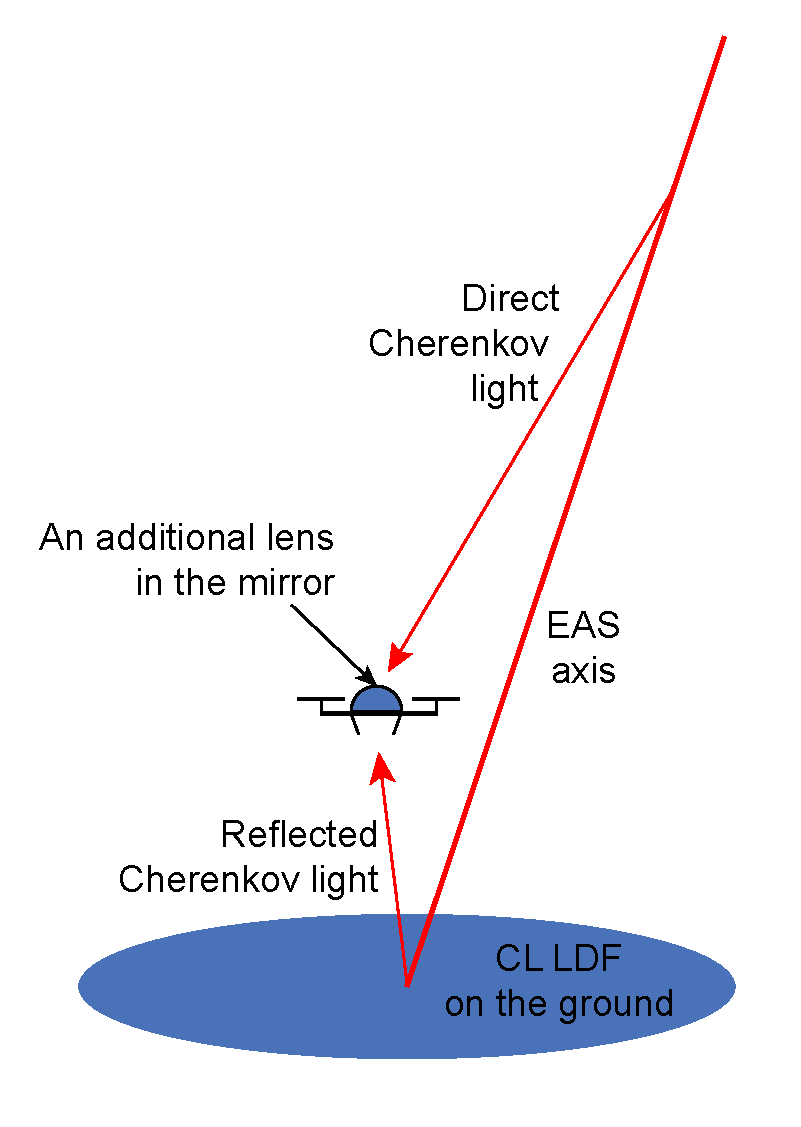
\includegraphics[height=.35\textheight]{DirectCL.pdf}
\caption{Scheme of direct and reflected Cherenkov light of EAS.}
\label{fig:DirectCL}
\end{figure}



\section{Advantages of the method}

\todoi{Этот текст повотряет текст предыдущей статьи}
The method of reflected CL detection has the following advantages over traditional EAS detection methods:
\begin{itemize}
\item The method provides a significant area of CL detection using a compact device;
\item Accurate estimation of PCR energy in an individual event thanks to the quasi-calorimetric method of energy detection;
\item The field of view of individual sensitive elements of the device covers a significant part of the surveyed area, what allows to observe the EAS CL near the shower axis, usually inaccessible to ground-based CL detector arrays. This circumstance significantly increases the accuracy of the primary particle type estimation;
\item Allows to measure the same PCR energy range with different resolution (distance between the centres of the fields of view of neighbouring sensory elements) by variating the elevation of the detector, thus allowing to control the magnitude of systematic errors;
\item The small size of the required detector allows to combine the calibration techniques accessible currently only to imaging air Cherenkov telescopes (direct calibration) with large scale measurements that are accessible only for conventional ground-based arrays;
\item Precise timing and high level of synchronization for better primary particle arrival direction reconstruction what has a direct impact on the precision of the EAS energy estimation.
\item The compact and tight arrangement of the detector electronics and sensitive elements allows the use of complex local topological trigger conditions that can greatly decrease random coincidences thus allowing to lower the energy threshold for the measurements.
\end{itemize}



\begin{figure}[t]
\centering % \begin{center}/\end{center} takes some additional vertical space
\hfill
\includegraphics[height=.25\textheight]{sphere2spectrum.pdf}
\hfill
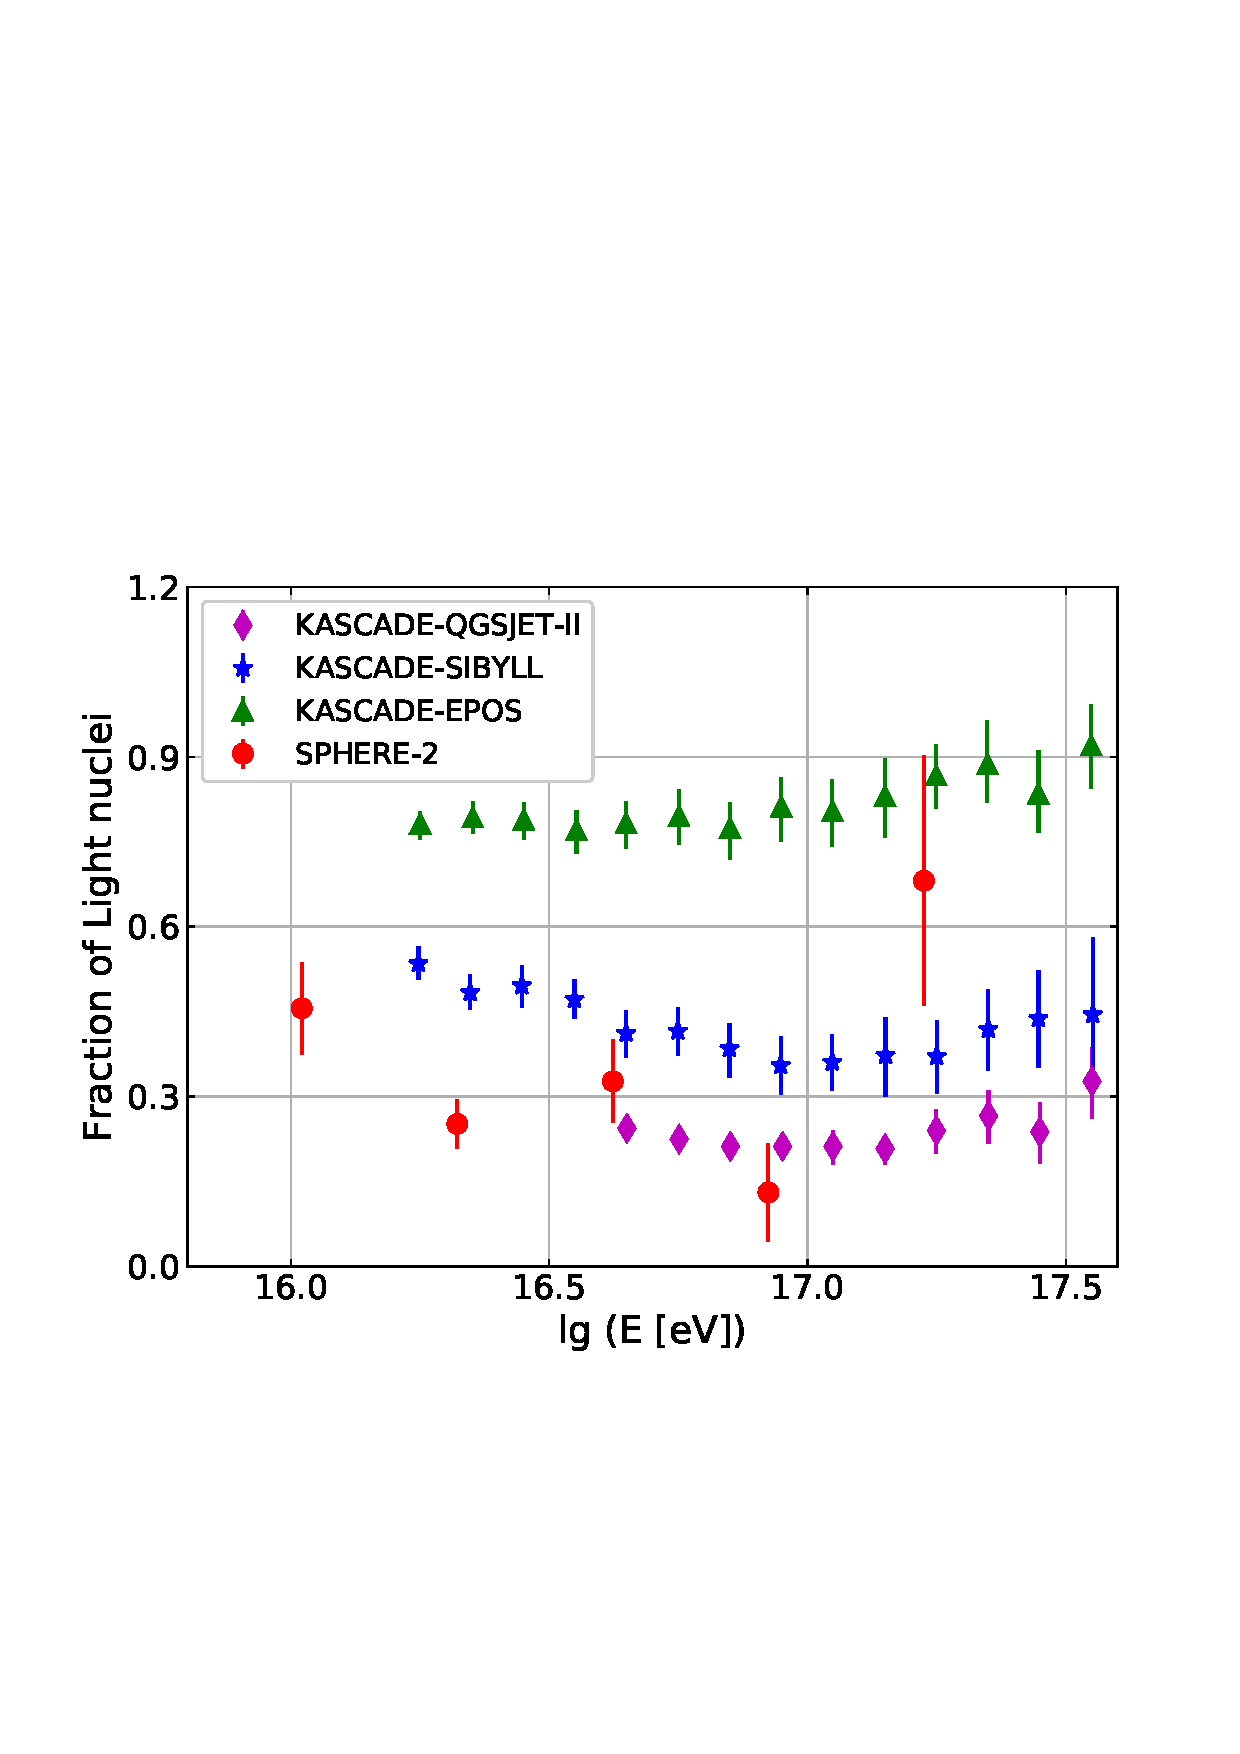
\includegraphics[height=.25\textheight]{sphere2composition.pdf}
\hfill
% "\includegraphics" from the "graphicx" permits to crop (trim+clip)
% and rotate (angle) and image (and much more)
\caption{Results of the SPHERE-2 experiment. On the left the energy spectrum of the PCR (red circles) is shown in comparison with the results of the Tunka-133~\cite{Tunka2020} (blue squares) and KASCADE Grande~\cite{Ape12} (green triangles) experiments. On the right the chemical composition estimates are shown (red circles) in comparison with the results of the KASCADE Grande experiment~\cite{Ape13}}
\label{fig:Sphere_results}
\end{figure}



\section{Detector Design}
It is planned to design a compact detector that will have the following characteristics:

The detector will use the Schmidt optical system. In this system, the central part of the mirror is not used since it is in the shadow of the photodetector. This area can be used by a system with approximate aperture of 100 cm2 for registration of the direct CL. Calculations show that for the EAS from 1 PeV proton the CL photons density is ~100 photons per cm at a distance of 100 m from the shower axis. Taking into account the SiPM quantum efficiency and losses on optical elements the expected number of registered photoelectrons is around 1000. The estimation of the primary particle mass can use the information on the intensity and angular properties of the direct CL in addition to the data on the reflected CL. It is assumed that the EAS from the primary proton should form a light spot different of Fe nuclei at the same primary energy and depth of EAS maximum.

\subsection{SiPM segment prototype }
The main sensitive element of the new detector will consist of 7-channel SiPM boards based on Micro FC-60035 SiPMs. The tests of a such boards were successfully completed. Each board was equipped with 7 preamplifiers and a temperature sensor. Each SiPM was equipped with a CA10929-Boom-MC-W light collector with and angular characteristic of $\pm$24 degrees at 50\% effectiveness. In this project, we plan to modify and adapt the SiPM board for use in a wide angle optical system.

\subsection{SiPM modelling}
(Left) An electronic circuity model approximating real SiPM. The circuit model was built in MATLAB Simulink. (Top) The model curve of current pulse from a single photoelectron obtained from MATLAB Simulink in comparison to the manufacturer provided curve.

\section{Experiment modelling}

Criterion value distributions for p, N, Fe primaries. 

Zenith angle: 15~$^\circ$. 
Atmosphere model: 11. 

Figures inside the panels denote the probabilities of misclassification (classification errors) for pairs of primary particles p-N and N-Fe.
a,b – E0 = 10PeV, 
c,d – E0 = 30PeV, 
a,c – h(elevation above the snowed surface) = 500m,
b,d – h = 900m.

\section{Conclusion}
The development of a new SiPM based detector for the EAS studied continues. A prototype of a photosensitive matrix element has been developed and is being tested. The detector design and feasibility of some technical solutions are being studied.  For this purpose, a SiPM circuit model with a fast output was created. The analysis of the detector design performance relative to the mass composition study is continued.

\section{Acknowledgments}
\todoi{Этот текст повотряет текст предыдущей статьи}
We warmly acknowledge the fundamental role in the development of reflected Cherenkov light detection method, pioneer works and important contributions to the project of our deceased colleague R.A.~Antonov.

\section{References}
\bibliography{TIPP_Sphere}

\end{document}